\chapter{Uvod}

U ovom poglavlju prikazane su neke od funkcije koje se mogu koristiti prilikom
oblikovanja rada i prikaza rezultata istraživanja korištenjem \LaTeX a.

\section{Matematički izraz}


Primjer matematičke formule prikazan je izrazom

\begin{equation}
  T: \mathbf{x}_B \mapsto \mathbf{x}_A \Leftrightarrow T(\mathbf{x}_B) = \mathbf{x}_A.
  \label{eq:transformacija}
\end{equation}


\section{Slika}


Slika \ref{fig:roc_example} služi kao primjer ubacivanja slike u tekst.

\begin{figure}
  \centering
  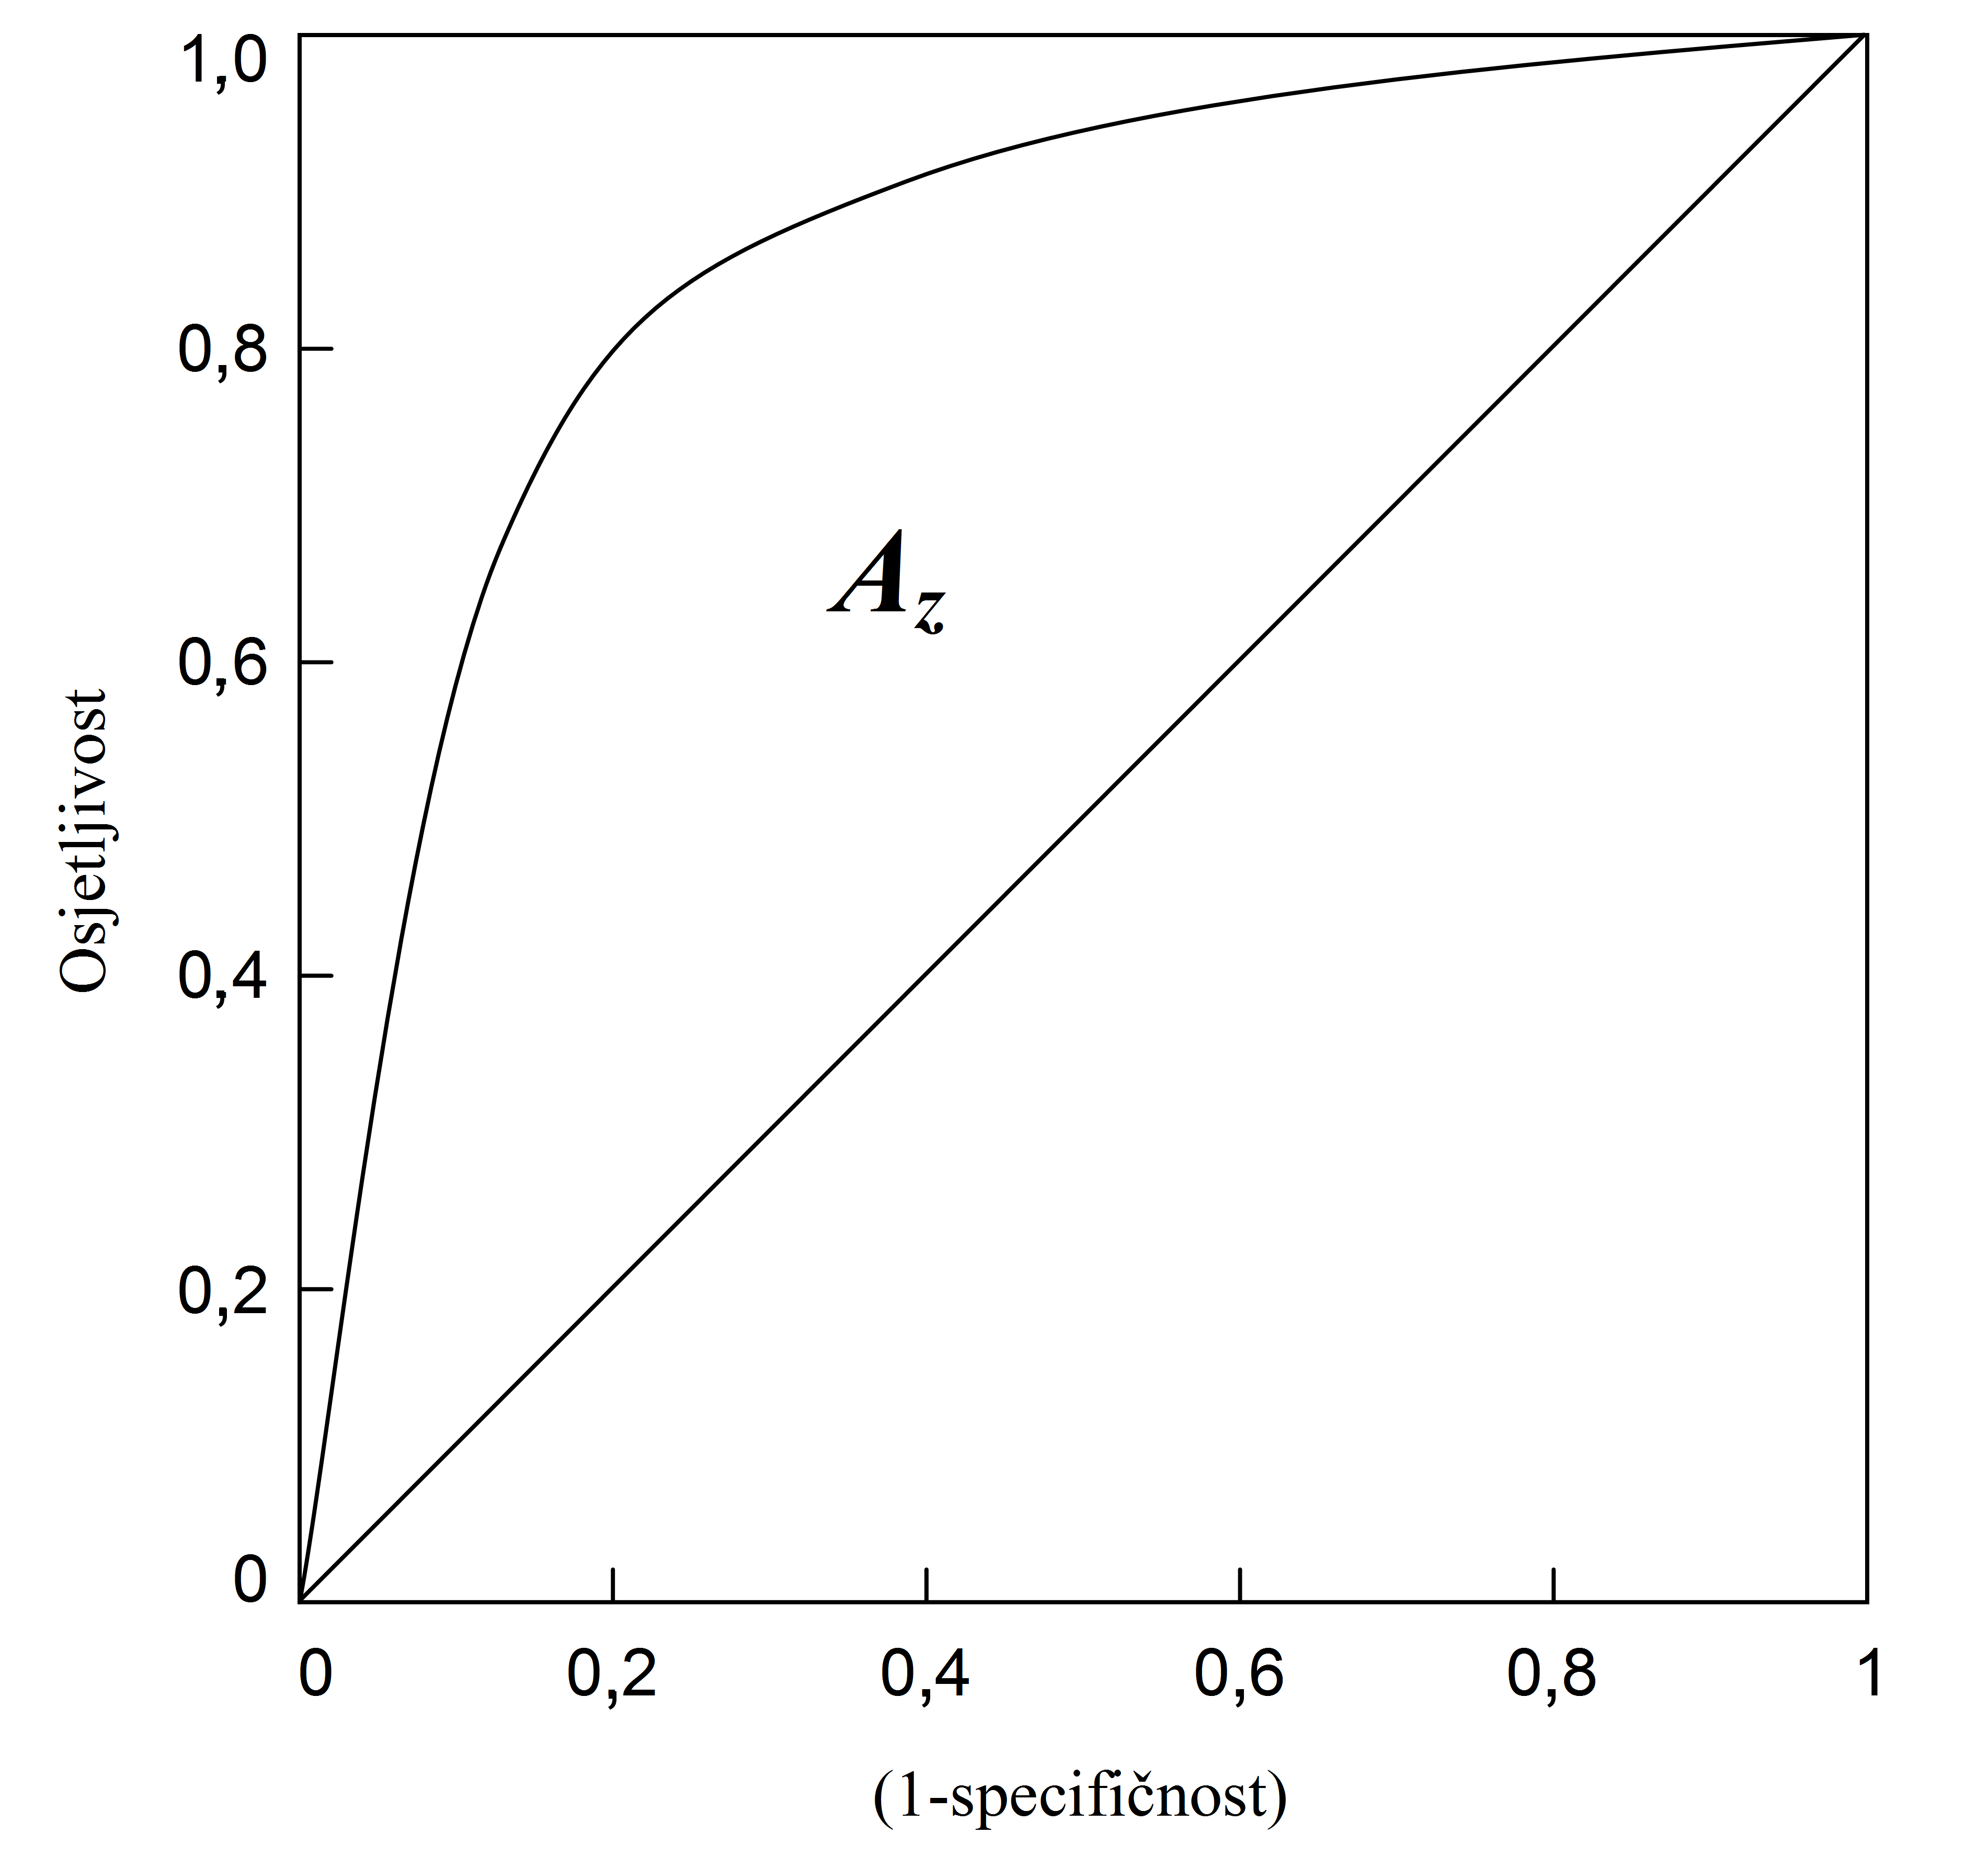
\includegraphics[width=0.7\textwidth]{roc_example}
  \caption{Primjer krivulje ROC}
  \label{fig:roc_example}
\end{figure}


\section{Tablica}


Formiranje tablice prikazano je na primjeru matrice podudarnosti u Tablici
\ref{tab:confusion_matrix}.

\begin{table} [!ht]
  \caption{Matrica podudarnosti}
  \centering  
  \begin{tabularx}{0.5\textwidth}{ c  c | c | c |}

    \cline{3-4}
    & & \multicolumn{2}{c|} {Predviđeno (\textit{predicited})}  \\ \cline{3-4}
    & & Negativno & Pozitivno \\ \cline{1-4}
    \multicolumn{1}{ |c } {\multirow{2}{*}{\rotatebox{90}{\parbox[c]{1.4cm} {Stvarno \\ (\textit{actual})}}}}  & \multicolumn{1}{ |c| }{Negativno} & NN & LPN \\ \cline{2-4}
    \multicolumn{1}{ |c  }{} & \multicolumn{1}{ |c| }{Pozitivno} & LNN & PN \\ \cline{1-4}

  \end{tabularx}
  \label{tab:confusion_matrix}
\end{table}

\subsection{\textit{Landscape}}

Postavljanja stranice u prikaz \textit{landscape} prikazano je umetanjem Tablice \ref{tab:mean_mias} u \textit{landscape}. Prikazano je i dodavanje \textit{footnotea} u tablicu.

\begin{landscape}
  \begin{table}
    % tekst u uglatim zagradama koje slijede \caption prikazuje se u Popisu tablica, a tekst u vitičastim zagradama koje slijede \caption prikazuje se iznad same tablice
    \caption[Srednje vrijednosti mjera sličnosti slika za bazu
	  mini-MIAS]{Srednje vrijednosti mjera sličnosti lijevog i desnog
	  mamograma prije i poslije registracije vođene različitim funkcijama
	  troška. Rezultati su prikazani za asimetrične (A) i normalne (N)
	  slučajeve u bazi mini-MIAS.}
    \begin{minipage}{\linewidth}   %minipage adjusts for its own footnotes
      \setcounter{mpfootnote}{\value{footnote}}
      \renewcommand{\thempfootnote}{\fnsymbol{mpfootnote}} 
      % \makebox[\textwidth] {          % center table on the page since it's wider than the page margins
      \newcolumntype{C}{>{\centering\arraybackslash}X}%
      \begin{tabularx} {\linewidth}{l C C C C C C C C C C C C} %{ c c c c c c c c c c c c c} 
        \multirow{2}{*}{\textbf{Mini-MIAS}} & \multicolumn{2}{c}{\textbf{SSD}} & \multicolumn{2}{c}{\textbf{CC}} & \multicolumn{2}{c}{\textbf{MI}} & \multicolumn{2}{c}{\textbf{NMI}} & \multicolumn{2}{c}{\textbf{SSIM}} & \multicolumn{2}{c}{\textbf{KLD}} \\  \cline{2-13}
        & \multicolumn{1}{c}{\textbf{A}} & \multicolumn{1}{c}{\textbf{N}} & \multicolumn{1}{c}{\textbf{A}} & \multicolumn{1}{c}{\textbf{N}} & \multicolumn{1}{c}{\textbf{A}} & \multicolumn{1}{c}{\textbf{N}} & \multicolumn{1}{c}{\textbf{A}} & \multicolumn{1}{c}{\textbf{N}} & \multicolumn{1}{c}{\textbf{A}} & \textbf{N} & \multicolumn{1}{c}{\textbf{A}} & \multicolumn{1}{c}{\textbf{N}} \\ \cline{1-13} %\hline

        Prije reg.  & 797,01 & 765,67  & 0,93 & 0,92 & 0,86 & 0,80 & 1,19 & 1,21 & 0,84 & 0,87 & 0,21 & 0,14 \\ \cline{1-13}
        Reg. sa SSD & 706,37 & 556,18  & 0,94 & 0,94 & 0,91 & 0,88 & 1,20 \footnotemark[1] & 1,24 \footnotemark[1] \footnotemark[2] & 0,86 \footnotemark[1] & 0,89 \footnotemark[1] & 0,20 & 0,14 \\ \cline{1-13}
        Reg. s CC   & 691,18 & 520,68  & 0,94 & 0,95 & 0,91 & 0,87 & 1,20 \footnotemark[1] & 1,23 \footnotemark[1] & 0,86 \footnotemark[1] & 0,89 \footnotemark[1] & 0,20 & 0,14 \\ \cline{1-13}
        Reg. s MI   & 840,84 & 649,41  & 0,92 & 0,93 & 0,92 & 0,87 & 1,21 \footnotemark[1] & 1,23 \footnotemark[1] & 0,86 \footnotemark[1] & 0,88 \footnotemark[1] & 0,20 & 0,14  \\ \cline{1-13}
        Reg. s NMI  & 758,53 & 572,00  & 0,93 & 0,94 & 0,92 & 0,86 & 1,21 & 1,23 & 0,86 \footnotemark[1] & 0,88 \footnotemark[1] & 0,20\footnotemark[2] & 0,14 \\ \cline{1-13}

      \end{tabularx} 
      \footnotetext[1]{statistički značajna razlika između asimetričnih i normalnih slučajeva za istu mjeru sličnosti}
      \footnotetext[2]{statistički značajna razlika u odnosu na vrijednost prije registracije za istu mjeru sličnosti} 
      % }
      \label{tab:mean_mias}
      \setcounter{footnote}{\value{mpfootnote}}
    \end{minipage}
  \end{table}
\end{landscape}


\section{Primjeri literature}

Popis literature navodi se na kraju doktorskog rada. Primjeri navođenja
literature su knjiga \cite{Hajn01}, poglavlje u knjizi \cite{Samp05}, članak
objavljen u časopisu \cite{Sim03}, članak objavljen na konferenciji
\cite{Wirt99}, doktorski rad \cite{Will93}, Internetski izvor \cite{Jone12} te
različite druge publikacije \cite{Rsoft}. Stil navođenja literature temelji se
na stilu razvijenom za IEEE časopise i konferencije, autora Michaela Shella uz
unesene prilagodbe stila za doktorski rad pisan na FER-u.
